%----------------------------------------------------------------------------------------
%	PACKAGES AND DOCUMENT CONFIGURATIONS
%----------------------------------------------------------------------------------------

\documentclass{article}

\usepackage[version=3]{mhchem} % Package for chemical equation typesetting
\usepackage{siunitx} % Provides the \SI{}{} and \si{} command for typesetting SI units
\usepackage{graphicx} % Required for the inclusion of images
\usepackage{natbib} % Required to change bibliography style to APA
\usepackage{amsmath} % Required for some math elements 
\usepackage{enumitem}% For lists
\usepackage{mathptmx}% For textbf
\usepackage{float} %for correct image placement
\usepackage{textcomp} % for texttildelow
\usepackage[T1]{fontenc} % allows use of less than <
\usepackage{booktabs} % for tables


\setlength\parindent{0pt} % Removes all indentation from paragraphs

\renewcommand{\labelenumi}{\alph{enumi}.} % Make numbering in the enumerate environment by letter rather than number (e.g. section 6)

%\usepackage{times} % Uncomment to use the Times New Roman font

%----------------------------------------------------------------------------------------
%	DOCUMENT INFORMATION
%----------------------------------------------------------------------------------------

\title{M152A - Lab 3 \\ Stopwatch} % Title

\author{Markus \textsc{Notti} - 904269231 \\ Kyle \textsc{Baker}  - 604273748 \\ Niels \textsc{Pineda} - 604272353} % Author name


\date{\today} % Date for the report

\begin{document}

\maketitle % Insert the title, author and date

%----------------------------------------------------------------------------------------
%	SECTION 1
%----------------------------------------------------------------------------------------

\section*{Introduction}

%Summarize background information
%about the lab and the detailed design requirements. It?s very important to
%make sure you are designing the right thing before starting.

In this lab, we implemented a basic stopwatch, and in the process, went through the complete FPGA design flow. This stopwatch is capable of counting seconds and minutes up to 99 minutes, and displaying the time on a seven segment display. We also designed the stopwatch with pause, adjustment, and direction capabilities.  

The stopwatch itself was designed with 5 primary inputs: ADJ, SEL, DIR, PAUSE, and RESET.\\

ADJ was controlled by a switch that, when set high, would put the stopwatch in adjustment mode, meaning that the stopwatch would count at a rate of 2 Hz, and depending on SEL, and DIR, either only the minutes or only the seconds would change.  This adjustment mode is the way for a user to change the stopwatch's value to a desired value. \\

\begin{figure}[H]

\begin{center}
\begin{tabular}{ | c | c | }
\hline
\textbf{ADJ} & \textbf{Action} \\ 
\hline
0 & Stopwatch counts normally\\
\hline
1 & Stopwatch enters adjustment mode and counts at 2 Hz\\
\hline
\end{tabular}

\caption{ADJ Switch}

\end{center}
\end{figure}


SEL was controlled by another switch, which when set high would change seconds in adjustment mode, and when set low would change minutes in adjustment mode.  Note that if ADJ is set to low, the value of SEL makes no difference.\\

\begin{figure}[H]
\begin{center}
\begin{tabular}{ | c | c | }

\hline
\textbf{SEL} & \textbf{Action} \\ 
\hline
0 & During adjustment mode, minutes change at rate of 2 Hz\\
\hline
1 & During adjustment mode, seconds change at rate of 2 Hz\\
\hline

\end{tabular}
\caption{SEL Switch}
\end{center}
\end{figure}

DIR was controlled by yet another switch, which when set high, would cause the stopwatch to count up from zero, and when set to low would cause the stopwatch to count down to zero.  Note that this direction controls the direction of the counting regardless of whether or not the stopwatch is in adjustment mode or not. \\

\begin{figure}[H]
\begin{center}
\begin{tabular}{ | c | c | }

\hline
\textbf{DIR} & \textbf{Action} \\ 
\hline
0 & Stopwatch counts down to zero\\
\hline
1 & Stopwatch counts up from zero\\
\hline

\end{tabular}
\caption{DIR Switch}
\end{center}
\end{figure}

PAUSE was controlled by a button, which when pressed would pause the stopwatch.  In order to filter out noise and correctly pause the stopwatch, we had to implement debounce logic for this functionality which will be talked about in the design section of the lab.\\

RESET was controlled by another button, which when pressed would reset the stopwatch's count to 00:00.\\

While taking 5 inputs, the stopwatch had one output, the seven segment display.  This output, however, was a little bit more complex than a single output.  The seven segment display was split into 4 digits and 8 segments per digit (really making it a 32 segment display).  The main challenge we had to deal with when outputting the correct time on the display was the fact that you could only send 1 combination of segments to the display. This meant that if I wanted to display separate numbers on different digits, I could not physically do it.  With the segmented display we used on our board, it is physically impossible to display two different numbers on two different digits.\\ 
To get around this, we displayed one digit every time a 500 Hz clock was high, cycling through all four of the digits more than 125 times a second.  This gave the illusion that the segmented display was displaying 4 different numbers simultaneously, though it wasn't really.

 
%----------------------------------------------------------------------------------------
%	SECTION 2
%----------------------------------------------------------------------------------------

\section*{Design Description}

%Design description (15%). Document the design aspects including the basic
%description of the design, modular architecture, interactions among the
%modules, and interface of each major module. You should include schematics
%for the system architecture. You can also include figures for state machines
%and Verilog code when needed.

% TODO: Make circuit diagram
% TODO: Make sure the figures referenced are correct

When designing the lab, we created two main modules, clock and stopwatch.  The clock module created slower clocks to regulate other parts of the program, while the stopwatch module held the majority of the program logic. Within the stopwatch module, we will specifically talk about the debounce logic used to filter noise on pause clicks, and also the logic behind the two separate clocks regulating the two always blocks.

\subsection*{Clock Module}

The clock module took as input a 100 MHz clock and outputted two separate clocks to govern the rest of the program: a 2 Hz clock and a 500 Hz clock.  This was implemented by 2 simple counters. The 2 Hz counter would count to 50,000,000, and the 500 Hz clock would count to 200,000.  At the posedge of the 10 MHz clock, the counts would increment until they reached their respective maximums, triggering the appropriate output clocks to 1. After reaching this maximum value, the counters would drop back to zero and start their counts over again.  This clock module was the beating heart of our software, controlling the rates at which all logic would be calculated, all input would be read and all output would be written.

\subsection*{Stopwatch Module}

Our stopwatch module held the main logic for our program. This module was governed by two separate clocks, the output clocks from the clock module, and the functionalities that each one of those clocks defined were placed into their own respective always blocks looking for their respective clocks to hit posedge. In this module, the main functionality that had to be implemented was the counting of seconds and minutes to be displayed on the stopwatch, the displaying of digits on the seven segment display, and appropriately responding to input.

\subsection*{Counting Time - 2 Hz Clock}

The 2 Hz clock controlled the logic for updating the stopwatch's minutes and seconds count.  We started by having 2 separate clocks, a 1 Hz clock and a 2 Hz clock, one to govern when the stopwatch was in normal mode, and the other to govern when the stopwatch was in adjust mode, however, it proved less complicated to go with a single 2 Hz clock. It would simply increment a minutes and seconds count every other time the posedge was hit while in normal mode, thus mimicking a 1 Hz clock.  When adjustment mode was enabled, however, the time on the stopwatch would be updated every time the clock hit posedge, meaning that it would truly update at a rate of 2 Hz.  \\

On this 2 Hz posedge, the stopwatch module also takes care of translating the minutes count and the seconds count to 4 binary representations ready to be output to the seven segment display. These 4 binary encodings, one for each digit, are calculated by a priority encoder and then are stored in registers that can be accessed by the second clock governing the stopwatch module: the 500 Hz clock.

\subsection*{Displaying Digits - 500 Hz Clock}

The 500 Hz clock in the stopwatch module is primarily responsible for displaying the appropriate digits on the seven segment display.  This task is taken care of by cycling through the 4 digits on the segmented display.  Since each of the appropriate binary encodings for each of the digits is already calculated and stored by the 2 Hz clock, the 500 Hz clock simply has to cycle through the 4 digits, displaying 1 of them every 1/500th of a second.  This is simply done with a modulus, and displays the digits too fast for the human eye to pick up the flicker from any of the digits as they flash on to off to on.

\subsection*{Debounce Logic}

Another critical feature we had to implement in order to get our pause button working correctly was debounce logic.  Debouncing is a phenomenon that occurs when a user clicks a button triggering 1's to be sent to that particular input.  However, this stream of high logic is interrupted by fluctuating patterns of zeros and ones.  It is never usually as simple as 1 high triggered by user input.  Therefore, without debounce logic, if a user presses a pause button, the stopwatch could pick up any combination of ones and zeros, pausing and unpausing the stopwatch many times, before finally settling on a paused or unpaused state (which could be correct or not). \\

To implement our debounce logic, we added another counter to our clock module, which took as input the pause button, in addition to the 100 MHz clock.  The program then, inside the clock module, checks if the pause button is high.  If high, it increments a counter until a value of 3,000,000 is reached.  If the max value has been reached and the pause button input is still high, in other words, if the pause button remains high for 3,000,000 counts of the 100 MHz clock (3/10 of a sec), then the counters in the clock module stop, stopping all logic.  The stopwatch effectively freezes in pause mode until the same sustained high is measured as input from the pause button, thereby resuming the clocks and resuming the stopwatch.


%----------------------------------------------------------------------------------------
%	SECTION 3
%----------------------------------------------------------------------------------------

\section*{Simulation}

%Simulation documentation (10%). Document all the simulation efforts (what
%requirements are tested and what the test cases are), document bugs found
%during simulation, and provide simulation waveforms. Include all simulation
%testbench code source files.

The simulation portion of the lab involved several test bench files, one for each individual module, with the most thorough of the test cases falling under the overarching FPCVT.  By understanding what each module was intended to do, and thus knowing the expected output for each one, the testing simply consisted of: creating a test bench file via adding a ``testing fixture'' source, then writing example instances along with a delay in said file, and finally running through the iSIM Waveform while checking accuracy by hand. Our individual modules, which more or less acted as ``sub/helper-functions'' in order to implement the overall module of FPCVT, consisted of: convertToSignMag, countLeadZeros, extractLeadBits, and rounding.  While it may not have been the best idea, we made very simple and basic test cases for these smaller modules in order to allow us to continue to progress in a timely fashion, while still working at a timely rate.  \\ 

For convertToSignMag, the input was the input data in the form of two's complement.  The two instantiations we tested were the integer values of 1 and -1, or D2 = 12'b000000000001 and D2 = 12'b111111111111 respectively.  We felt as though these were good, simple test cases as they were several corner cases which also tested if both our negative and positive conversion was working correctly.  As expected, the outcomes were correctly stored in S and MAG: for 1 S=0 and MAG=00000000001 and for -1 S=1 and MAG=00000000001.     

\begin{figure}[H]
	\begin{center}
		%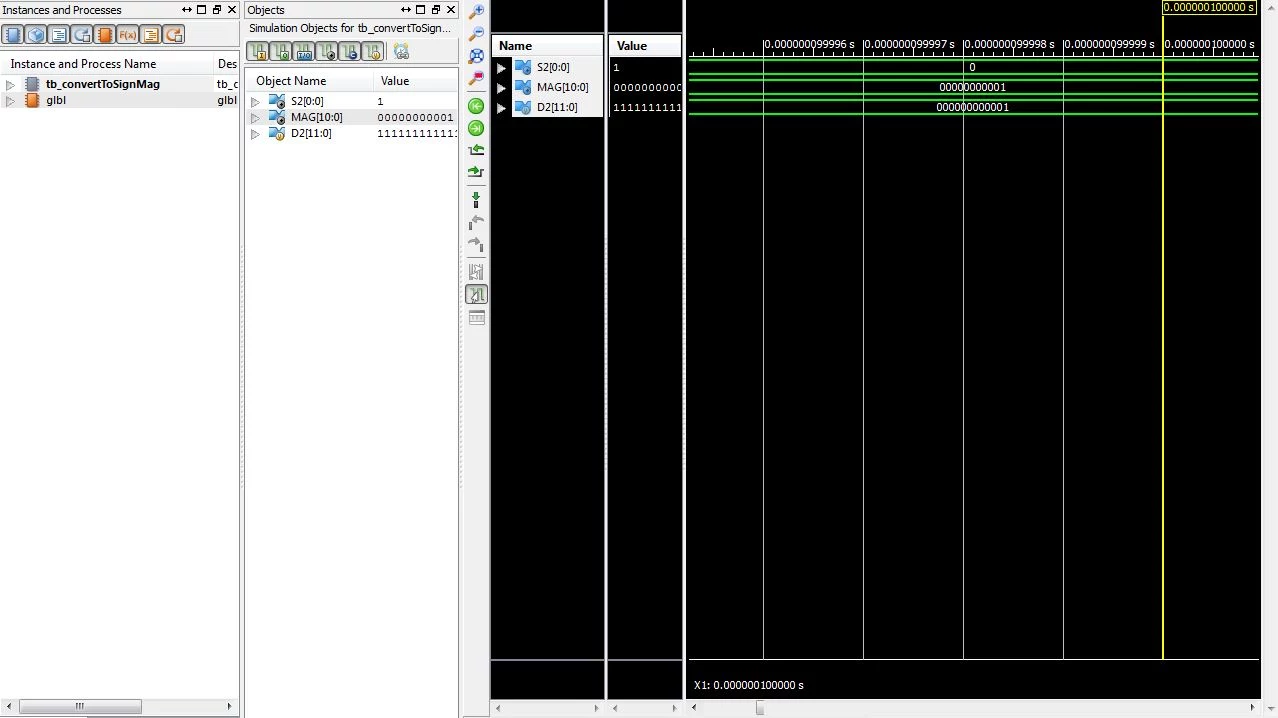
\includegraphics[width=1.2\textwidth]{sim1.png} 
		\caption{Example testbench simulation testing convertToSignMag module}
	\end{center}
\end{figure}

The following simulation for countLeadZeros was by far the trickiest for our group, as we initially had trouble understanding exactly what the output was to look like; consequently, this led to us believing our first attempt was correct which made our overall converter fail.  However, after clarifying the process for this module, we were able to produce the correct output, in which we checked many cases including: MAG3 = 11'b00000000000; MAG3 = 11'b00000000001; MAG3 = 11'b00000000010; MAG3 = 11'b00000000100; MAG3 = 11'b00000001000; MAG3 = 11'b00000010000; MAG3 = 11'b00000100000; MAG3 = 11'b10100100000; and MAG3 = 11'b11111111111.  Our initial approach led to undefined behavior, but after the fix, we were very thorough in testing this module.  All of these test cases simply represented every different number of leading zeros (from 0 to > 8) which would led to different exponents.

\begin{figure}[H]
	\begin{center}
		%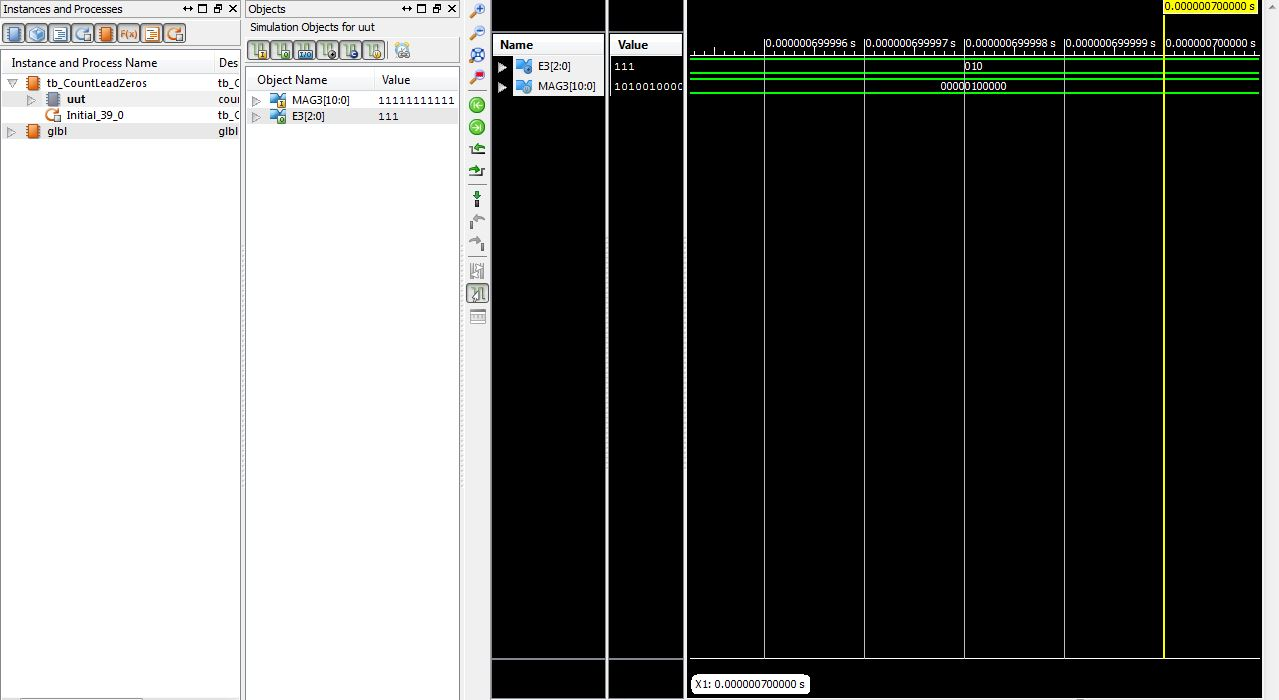
\includegraphics[width=1.2\textwidth]{sim2.png} 
		\caption{Example testbench simulation testing countLeadingZeros module}
	\end{center}
\end{figure}

Module extractLeadBits was relatively straightforward, and similarly, so were the test cases.  Because of the simplicity of the code itself, which merely consisted of a priority encoder, we only used two test cases, which were passing in the magnitude (MAG4) as MAG4 = 11'b01101000101 and MAG4 = 11'b00000101111.  These represented relatively simple cases that assured our priority encoder was working, and both of these resulted in the expected outcomes.


\begin{figure}[H]
	\begin{center}
		%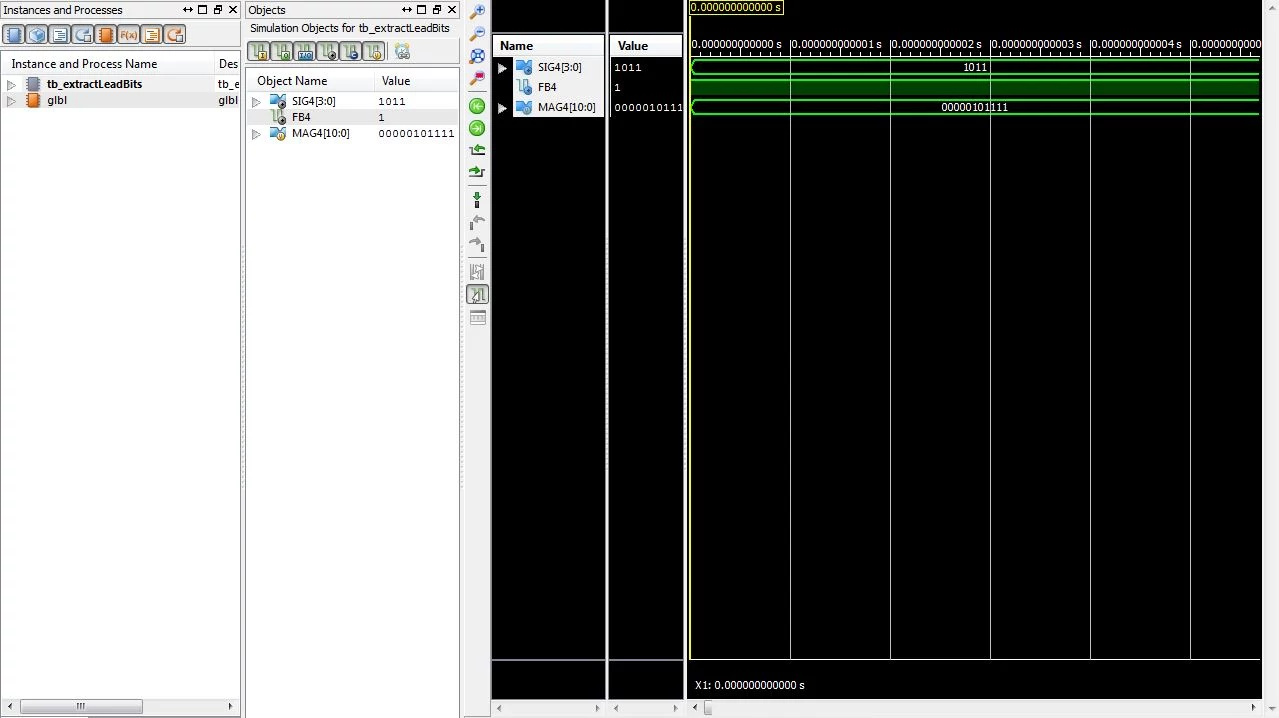
\includegraphics[width=1.2\textwidth]{extractLeadingBitsSim.png} 
		\caption{Example testbench simulation extractLeadBits module}
	\end{center}
\end{figure}


The final module (aside from the converter) was used for rounding of the floating point conversion.  We carefully tested the various corner cases (in this case, the various types of overflow) after testing a couple of very basic cases.  The cases we tested were based off of changing the exponent (E5), significand (Sig5) and fifth-bit (FB5); the cases included: [E5 = 3'b001; SIG5 = 4'b0001; FB5 = 0;] ; [E5 = 3'b001; SIG5 = 4'b0001; FB5 = 1;] ; [E5 = 3'b001; SIG5 = 4'b1111; FB5 = 1;] and [E5 = 3'b111; SIG5 = 4'b1111; FB5 = 1;].  The first two instantiations were very simple cases, simply assuring if the basic rounding was correct.  Once those were verified, we tested two major overflow conditions, one in which the exponent could had room to carry over, and the other where there was no room for adding to any input.  These covered the major corner cases, all of which eventually passed with some adjustments to the code to account for those particular cases. 

\begin{figure}[H]
	\begin{center}
		%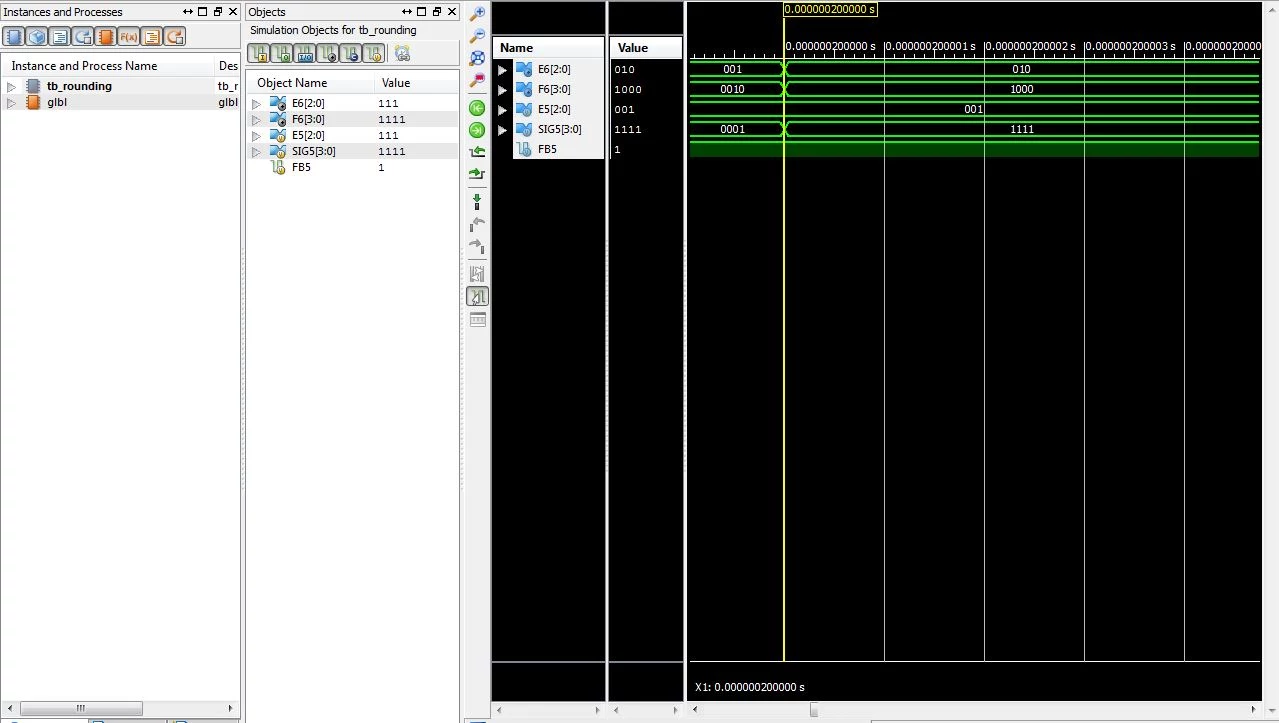
\includegraphics[width=1.2\textwidth]{sim5.png} 
		\caption{Example testbench simulation testing rounding module}
	\end{center}
\end{figure}

Lastly, and most importantly, we tested the entire converter, FPCVT.  The major trouble we had testing this came when we believed all of our sub-modules were working correctly, when in fact countLeadZeros was not outputting what it was supposed to.  After that adjustment, our test simulations were generally correct aside from a single corner case (which was the most negative number).  We had a variety of test cases including: D = 12'b 000000101100; D = 12'b 000000101101; D = 12'b 000000101110; D = 12'b 000000101111; D = 12'b 111111111111; D = 12'b 011111111111; D = 12'b 011111000000; D = 12'b 100000000000; D = 12'b 111001011010, where D was the input.  As indicated by the images below, these test cases checked for multiple conditions including: the base case of a generic number (000000101110), negative rounding (111001011010), negative one (111111111111), the most positive number (011111111111), and the edge case (which is the one we initially missed) of 100000000000. 

\begin{figure}[H]
	\begin{center}
		%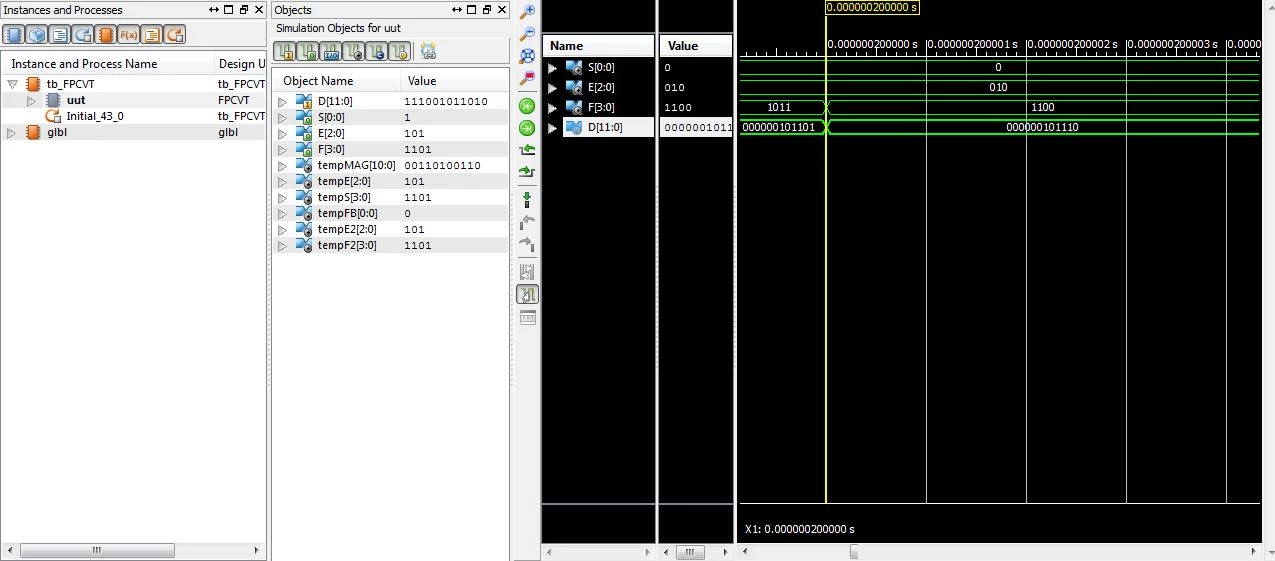
\includegraphics[width=1.2\textwidth]{sim3.png} 
		\caption{Example testbench simulation testing generic number on fpcvt module}
	\end{center}
\end{figure}

\begin{figure}[H]
	\begin{center}
		%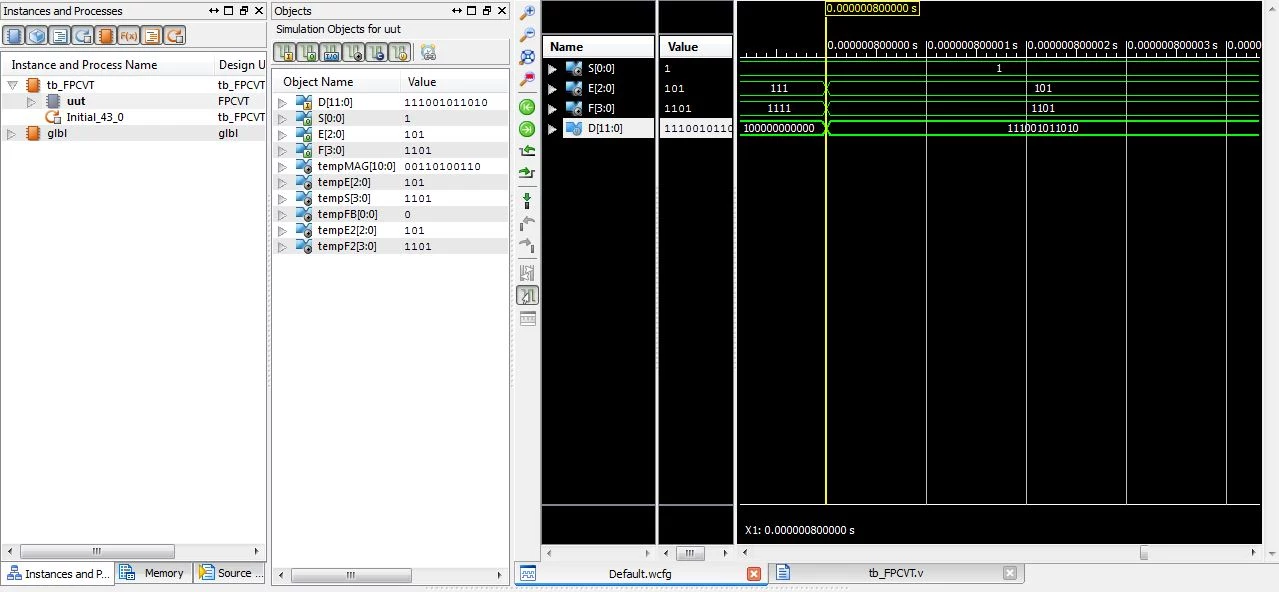
\includegraphics[width=1.2\textwidth]{sim4.png} 
		\caption{Example testbench simulation testing negative rounding on fpcvt module}
	\end{center}
\end{figure}

\begin{figure}[H]
	\begin{center}
		%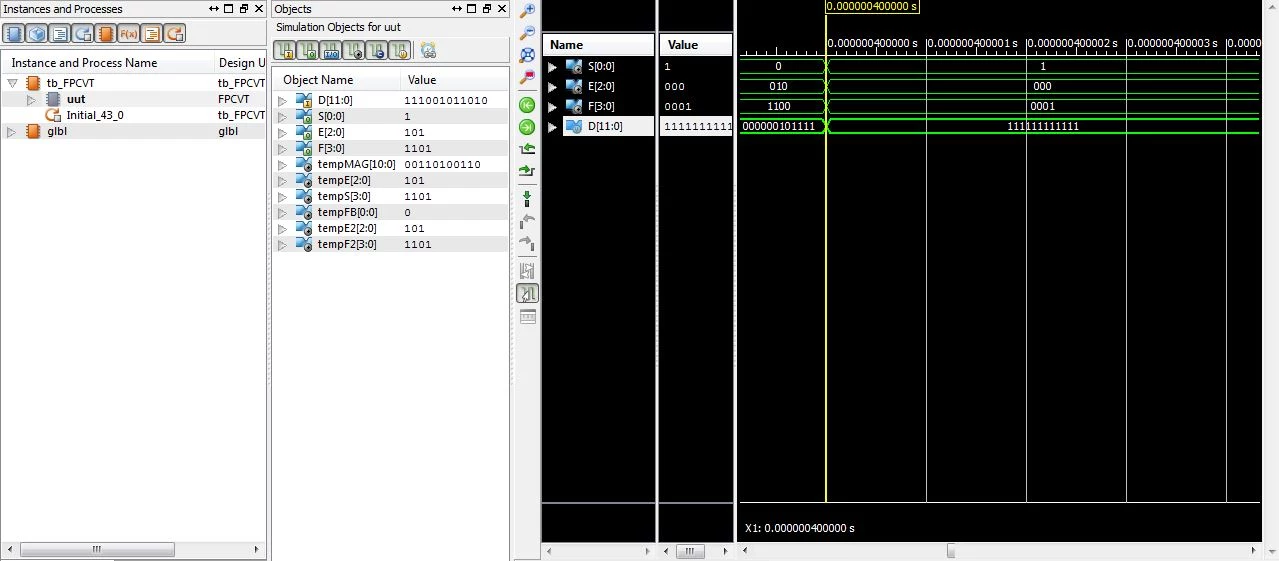
\includegraphics[width=1.2\textwidth]{sim7.png} 
		\caption{Example testbench simulation testing negative 1 on fpcvt module}
	\end{center}
\end{figure}

\begin{figure}[H]
	\begin{center}
		%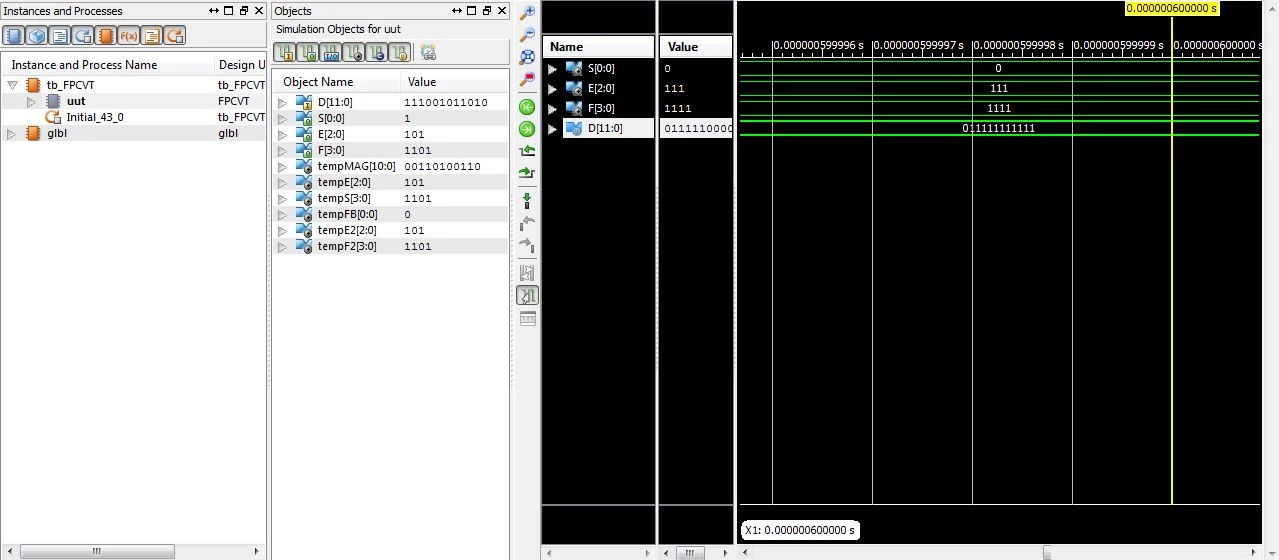
\includegraphics[width=1.2\textwidth]{mostPositiveSim.png} 
		\caption{Example testbench simulation testing most positive number on fpcvt module}
	\end{center}
\end{figure}

\begin{figure}[H]
	\begin{center}
		%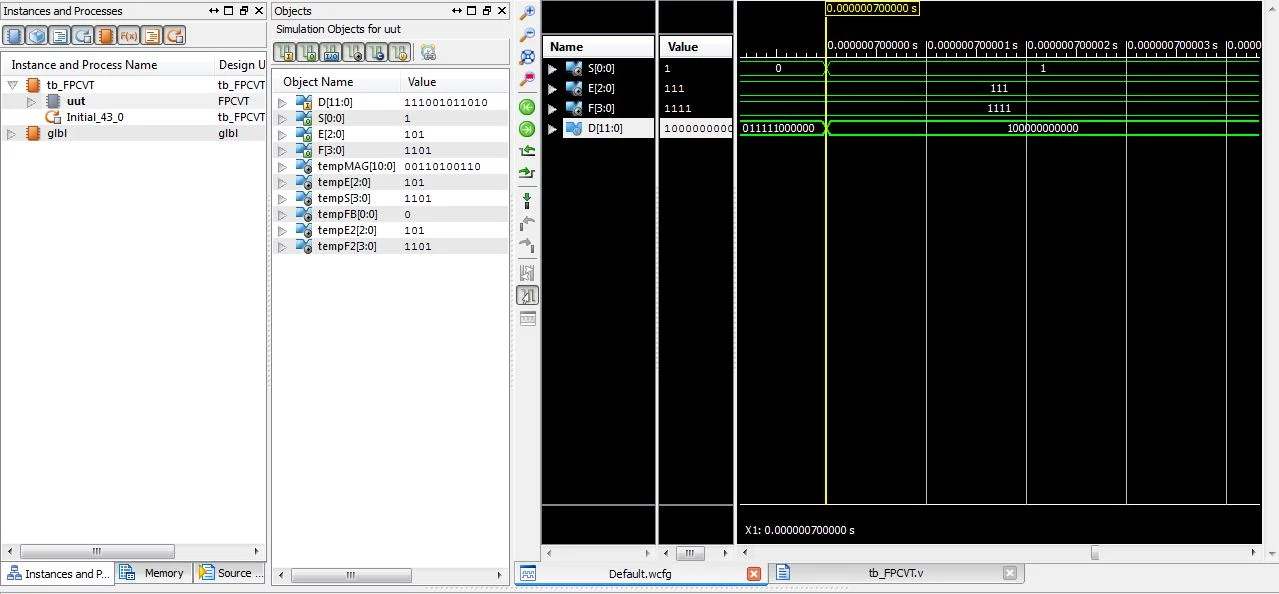
\includegraphics[width=1.2\textwidth]{sim6.png} 
		\caption{Example testbench simulation testing edge case on fpcvt module}
	\end{center}
\end{figure}

\section*{Conclusion}

%Conclusion (5%). Summary of the design. Difficulties you encountered, and
%how you dealt with them. General suggestions for improving the lab, if any.

Overall, the implementation of the converter went relatively smoothly, especially with the help of the lab manual.  By breaking down the the overall design and module of FPCVT into several modules, in our case: convertToSignMag, countLeadZeros, extractLeadBits, rounding, then using all of them in the, the process was made much clearer and easier.  Initially, we fed in the data in two's complement representation into the convertToSignMag.  That module's output was used as the input to countLeadZeros and extractLeadBits.  These output the exponent, significand, and fifth bit, which fed into the rounding process, which eventually led to the overall output. \\

There were, however, several difficulties throughout the implementation.  For starters, simply trying to understand Verilog, most notably when to use wires or registers along with dealing with assignments and always blocks, took a decent amount of time.  After understanding this and implementing our first module, we wrote our own test bench instead of simply adding a ``test fixture'' source file, which led to even more time being lost.  Our final problem with ISE came with a minor mistake, but we often would run the simulation on the uut file accidentally, which led to undefined behavior.  \\

Regarding the actual writing of code, the problems came from either counting the leading zeros or the various corner cases.  Most notably, the description in the lab manual for counting the leading zeros was worded oddly, which led to a confusion on what the module should actually do.  The only test case we initially failed was the case of 100000000000, but we were able to fix this in the convertToSignMag module. Aside from those issues, the lab was relatively straightforward.  



%----------------------------------------------------------------------------------------
%	BIBLIOGRAPHY
%----------------------------------------------------------------------------------------

%\bibliographystyle{apalike}

%\bibliography{sample}

%----------------------------------------------------------------------------------------


\end{document}